\section{Initial processing steps}

Diverse set of processing tasks: Preprocessing, segmentation, line separatino,
OCR, ...
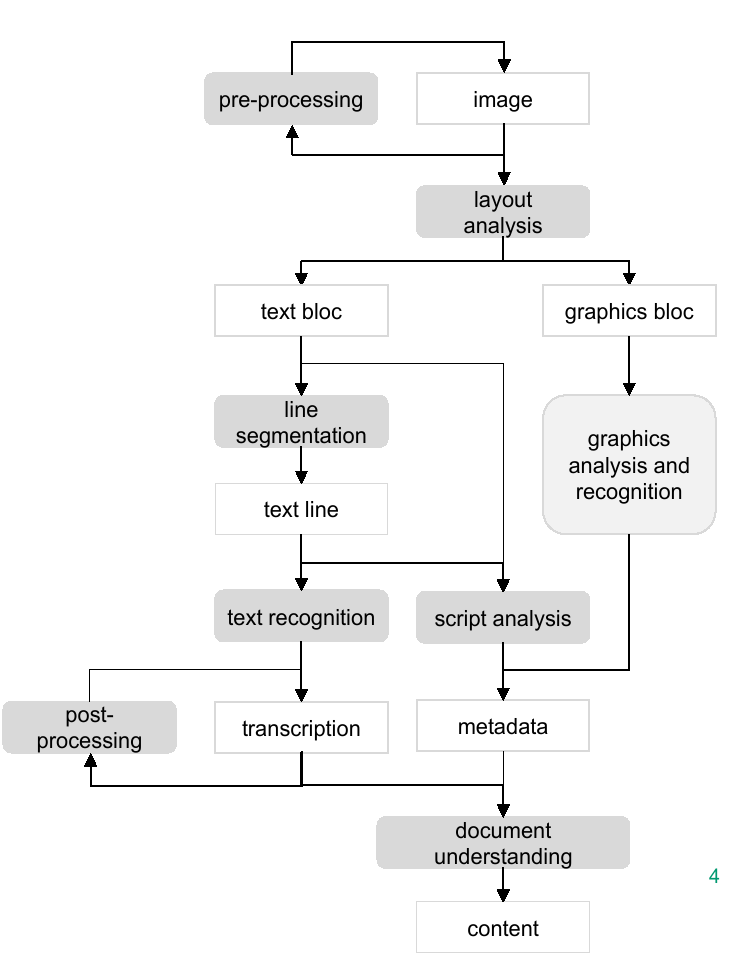
\includegraphics[width=0.5\textwidth]{resources/04_processing_chain}

\subsection{Preprocessing}

Improve quality of images for both visualization as well as processing.
Consists of adjusting resolution, sharpening, colour corrections, deskewing,
binarization, ...

\begin{description}
		\item[Hough transform] skew estimation by mapping pixels to 2D
				parameter space, polar coordinates to estimate skew angle.
		\item[Rotation] can be used to deskew, but introduces distortions
		\item[Bleedthrough] can be removed easily if backside known. Else, use
				gradients.
		\item[Binarization] Global and local operations
\end{description}

\subsection{Layout analysis}

Isolate text blocks, graphics, formula, images, ...

\begin{itemize}
		\item White streams detection (top-down) recursively does horizontal and vertical
				cuts through white areas. Works well for manhattan layout, less
				well for nested ones.
		\item Projection profiles (top-down) allow detecting columns or lines, requires
				unskewed image.
		\item Connected components (bottom-up), aggregation of connected
				components. Useful for binarized printed documents.
		\item Regional classification in e.g. historical documents.
\end{itemize}

\subsection{Text recognition}

\begin{itemize}
		\item OCR suitable for segmented printed text with high-quality images
		\item Handwriting recognition not yet mature, works decently on limited
				vocabulary or when training data available (rather than generic
				model)
		\item Binarization can introduce gaps which lowers OCR performance.
				Context-aware OCR can help, also with similar-looking
				characters.
		\item Sayre's paradox for cursive writing: Character recognition and
				segmentation dependant on each other. Workarounds include
				operations on full words, combining the two, or multiple
				attempts with the most likely one being used.
		\item Depending on alphabet, character recognition (Latin),
				dictionary-based word recognition (Arabic) or stroke
				recognition (Chinese, Japanese) applicable.
\end{itemize}

\subsection{Text alignment}

Align image of text with its transcript. Difficutly depends heavily on accuracy
of transcript and availability of linebreak information.

\subsection{Script analysis}

Script classification, language detection, font recognition, writer
identification, ...

Uses histograms of locale angle distribution, gradients, profiles, run lengths,
...

\subsection{Document understanding}

The last DIA step, first semantic step towards a specific application.
Transformation of physical to logical structure.

\subsubsection{Physical structure}

Publisher's point of view.

\begin{itemize}
		\item Organization of document into regions
		\item Regions into headings and text blocks
		\item Position of figures, separators, ...
\end{itemize}

\subsubsection{Logical structure}

Author's point of view.

\begin{itemize}
		\item Logical structure of document
		\item Articles, titles, headlines, paragraphs, ...
		\item Independent of presentation
\end{itemize}
